%----------------------------------------------------------------------------------------
%	PACKAGES AND OTHER DOCUMENT CONFIGURATIONS
%----------------------------------------------------------------------------------------

\documentclass[]{article}

\usepackage[italian]{babel}
\selectlanguage{italian}

%%%%%%%%%%%%%%%%%%%%%%%%%%%%%%%%%%%%%%%%%
% Lachaise Assignment
% Structure Specification File
% Version 1.0 (26/6/2018)
%
% This template originates from:
% http://www.LaTeXTemplates.com
%
% Authors:
% Marion Lachaise & François Févotte
% Vel (vel@LaTeXTemplates.com)
%
% License:
% CC BY-NC-SA 3.0 (http://creativecommons.org/licenses/by-nc-sa/3.0/)
% 
%%%%%%%%%%%%%%%%%%%%%%%%%%%%%%%%%%%%%%%%%

%----------------------------------------------------------------------------------------
%	PACKAGES AND OTHER DOCUMENT CONFIGURATIONS
%----------------------------------------------------------------------------------------

\usepackage{amsmath,amsfonts,stmaryrd,amssymb} % Math packages

\usepackage{enumerate} % Custom item numbers for enumerations

\usepackage[ruled]{algorithm2e} % Algorithms

\usepackage[framemethod=tikz]{mdframed} % Allows defining custom boxed/framed environments

\usepackage{listings} % File listings, with syntax highlighting
\lstset{
	basicstyle=\ttfamily, % Typeset listings in monospace font
}

%----------------------------------------------------------------------------------------
%	DOCUMENT MARGINS
%----------------------------------------------------------------------------------------

\usepackage{geometry} % Required for adjusting page dimensions and margins

\geometry{
	paper=a4paper, % Paper size, change to letterpaper for US letter size
	top=2.5cm, % Top margin
	bottom=3cm, % Bottom margin
	left=2.5cm, % Left margin
	right=2.5cm, % Right margin
	headheight=14pt, % Header height
	footskip=1.5cm, % Space from the bottom margin to the baseline of the footer
	headsep=1.2cm, % Space from the top margin to the baseline of the header
	%showframe, % Uncomment to show how the type block is set on the page
}

%----------------------------------------------------------------------------------------
%	FONTS
%----------------------------------------------------------------------------------------

\usepackage[utf8]{inputenc} % Required for inputting international characters
\usepackage[T1]{fontenc} % Output font encoding for international characters

\usepackage{XCharter} % Use the XCharter fonts

%----------------------------------------------------------------------------------------
%	COMMAND LINE ENVIRONMENT
%----------------------------------------------------------------------------------------

% Usage:
% \begin{commandline}
%	\begin{verbatim}
%		$ ls
%		
%		Applications	Desktop	...
%	\end{verbatim}
% \end{commandline}

\mdfdefinestyle{commandline}{
	leftmargin=10pt,
	rightmargin=10pt,
	innerleftmargin=15pt,
	middlelinecolor=black!50!white,
	middlelinewidth=2pt,
	frametitlerule=false,
	backgroundcolor=black!5!white,
	frametitle={Command Line},
	frametitlefont={\normalfont\sffamily\color{white}\hspace{-1em}},
	frametitlebackgroundcolor=black!50!white,
	nobreak,
}

% Define a custom environment for command-line snapshots
\newenvironment{commandline}{
	\medskip
	\begin{mdframed}[style=commandline]
}{
	\end{mdframed}
	\medskip
}

%----------------------------------------------------------------------------------------
%	FILE CONTENTS ENVIRONMENT
%----------------------------------------------------------------------------------------

% Usage:
% \begin{file}[optional filename, defaults to "File"]
%	File contents, for example, with a listings environment
% \end{file}

\mdfdefinestyle{file}{
	innertopmargin=1.6\baselineskip,
	innerbottommargin=0.8\baselineskip,
	topline=false, bottomline=false,
	leftline=false, rightline=false,
	leftmargin=2cm,
	rightmargin=2cm,
	singleextra={%
		\draw[fill=black!10!white](P)++(0,-1.2em)rectangle(P-|O);
		\node[anchor=north west]
		at(P-|O){\ttfamily\mdfilename};
		%
		\def\l{3em}
		\draw(O-|P)++(-\l,0)--++(\l,\l)--(P)--(P-|O)--(O)--cycle;
		\draw(O-|P)++(-\l,0)--++(0,\l)--++(\l,0);
	},
	nobreak,
}

% Define a custom environment for file contents
\newenvironment{file}[1][File]{ % Set the default filename to "File"
	\medskip
	\newcommand{\mdfilename}{#1}
	\begin{mdframed}[style=file]
}{
	\end{mdframed}
	\medskip
}

%----------------------------------------------------------------------------------------
%	NUMBERED QUESTIONS ENVIRONMENT
%----------------------------------------------------------------------------------------

% Usage:
% \begin{question}[optional title]
%	Question contents
% \end{question}

\mdfdefinestyle{question}{
	innertopmargin=1.2\baselineskip,
	innerbottommargin=0.8\baselineskip,
	roundcorner=5pt,
	nobreak,
	singleextra={%
		\draw(P-|O)node[xshift=1em,anchor=west,fill=white,draw,rounded corners=5pt]{%
		Question \theQuestion\questionTitle};
	},
}

\newcounter{Question} % Stores the current question number that gets iterated with each new question

% Define a custom environment for numbered questions
\newenvironment{question}[1][\unskip]{
	\bigskip
	\stepcounter{Question}
	\newcommand{\questionTitle}{~#1}
	\begin{mdframed}[style=question]
}{
	\end{mdframed}
	\medskip
}

%----------------------------------------------------------------------------------------
%	WARNING TEXT ENVIRONMENT
%----------------------------------------------------------------------------------------

% Usage:
% \begin{warn}[optional title, defaults to "Warning:"]
%	Contents
% \end{warn}

\mdfdefinestyle{warning}{
	topline=false, bottomline=false,
	leftline=false, rightline=false,
	nobreak,
	singleextra={%
		\draw(P-|O)++(-0.5em,0)node(tmp1){};
		\draw(P-|O)++(0.5em,0)node(tmp2){};
		\fill[black,rotate around={45:(P-|O)}](tmp1)rectangle(tmp2);
		\node at(P-|O){\color{white}\scriptsize\bf !};
		\draw[very thick](P-|O)++(0,-1em)--(O);%--(O-|P);
	}
}

% Define a custom environment for warning text
\newenvironment{warn}[1][Warning:]{ % Set the default warning to "Warning:"
	\medskip
	\begin{mdframed}[style=warning]
		\noindent{\textbf{#1}}
}{
	\end{mdframed}
}

%----------------------------------------------------------------------------------------
%	INFORMATION ENVIRONMENT
%----------------------------------------------------------------------------------------

% Usage:
% \begin{info}[optional title, defaults to "Info:"]
% 	contents
% 	\end{info}

\mdfdefinestyle{info}{%
	topline=false, bottomline=false,
	leftline=false, rightline=false,
	nobreak,
	singleextra={%
		\fill[black](P-|O)circle[radius=0.4em];
		\node at(P-|O){\color{white}\scriptsize\bf i};
		\draw[very thick](P-|O)++(0,-0.8em)--(O);%--(O-|P);
	}
}

% Define a custom environment for information
\newenvironment{info}[1][Info:]{ % Set the default title to "Info:"
	\medskip
	\begin{mdframed}[style=info]
		\noindent{\textbf{#1}}
}{
	\end{mdframed}
}
 % Include the file specifying the document structure and custom commands

\usepackage[T1]{fontenc}

\usepackage{imakeidx}
\makeindex[columns=3, title=Alphabetical Index, intoc]
\usepackage{hyperref}
\hypersetup{
    colorlinks,
    citecolor=black,
    filecolor=black,
    linkcolor=black,
    urlcolor=black
}

\usepackage{titling}
\renewcommand\maketitlehooka{\null\mbox{}\vfill}
\renewcommand\maketitlehookd{\vfill\null}

\usepackage{graphicx}
\graphicspath{ {./images/} }
\usepackage{subfig}
\usepackage{booktabs}
\usepackage{float}

\usepackage[notlot,notlof]{tocbibind}
\usepackage[super]{natbib}
\usepackage{url}

\usepackage{comment}
\usepackage{siunitx}
\newcommand{\Lagr}{\mathcal{L}}

%----------------------------------------------------------------------------------------
%	ASSIGNMENT INFORMATION
%----------------------------------------------------------------------------------------

\title{Formulario di Deep Learning} % Title of the assignment

\author{Mattia D'Urso} % Author name and email address

\date{Università degli Studi di Udine --- \today} % University, school and/or department name(s) and a date

%----------------------------------------------------------------------------------------

\begin{document}


%----------------------------------------------------------------------------------------
%	FIRST PAGE
%----------------------------------------------------------------------------------------



\begin{titlingpage}
\maketitle % Print the title
\end{titlingpage}



\addtocounter{page}{1}


\newenvironment{dedication}
  {%\clearpage           % we want a new page          %% I commented this
   \thispagestyle{empty}% no header and footer
   \vspace*{\stretch{1}}% some space at the top
   \itshape             % the text is in italics
   \raggedleft          % flush to the right margin
  }
  {\par % end the paragraph
   \vspace{\stretch{3}} % space at bottom is three times that at the top
   \clearpage           % finish off the page
  }


  \begin{dedication}
Al prof. Serra ,\par per avermi spinto incosapevolmente a scrivere questo formulario.
  \end{dedication}
%----------------------------------------------------------------------------------------
%	INDEX
%----------------------------------------------------------------------------------------


\phantomsection
\renewcommand{\contentsname}{Indice dei contenuti}
\tableofcontents


\clearpage


%----------------------------------------------------------------------------------------
%	CAPITOLO 1
%----------------------------------------------------------------------------------------



\section{Introduzione}
Questa raccolta di formule vuole essere un riassunto delle formule viste nel corso di Deep Learning 2020/2021 tenuto dal prof. Giuseppe Serra.

\subsection{Formule base}
\begin{figure}[h] 
\centering 
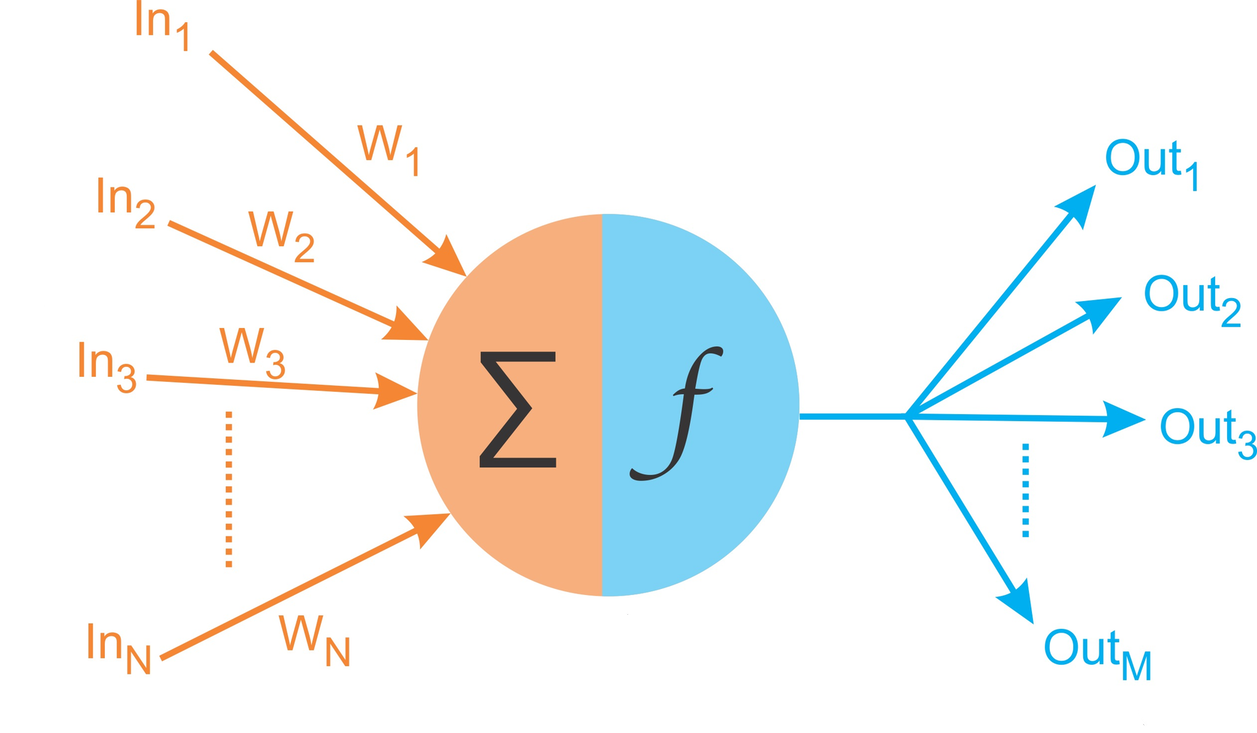
\includegraphics[scale=0.2]{dl} 
\end{figure}

\[h_{w,b}(X) = a = \sum_{} W^T X + b\]
\[ z = f(a)\] \\
con $f$ funzione di attivazione a piacere

%----------------------------------------------------------------------------------------

\subsection{Funzioni di attivazione}

Sigmoid function [0,1]\\
\[ Si(x) = \frac{1}{1+e^{-x}} \] \\

ReLU [0, x] \\ 
\[R(x) = max(0, x)\] \\

LeakyReLU [-x, x] con solitamente $\alpha = 0.2$ \\
\[ LR(x) = max(\alpha x, x)\]  \\

Softmax [0,1]  
\[ So(x) = \frac{e^{z_i}}{\sum_{j=0}e^{z_j}} \] \\

Tanh [-1, 1] \\
\[ Tanh(x) = \frac{e^{x} - e^{-x}}{e^{x} + e^{-x}}\]\\

%----------------------------------------------------------------------------------------

\subsection{Funzioni di costo/loss}
$y$ è la grand truth \\
$x$ sono gli input \\ 
$h_{w,b}(x_i)$ è la predizione\\


Mean Square Error (per la regression)\\

\[ \Lagr(w,b) = \frac{1}{m} \sum{(h_{w,b}(x_i) - {y_i})}^2 \] \\

Cross Entropy Loss (per la classificazione di più classi) \\
\[ \Lagr(w,b) = - \sum y_i ln(h_{w,b}(x_i)) \] \\

Binary Cross Entropy Loss (per una classificazione binaria) \\
\[ \Lagr(w,b) = - \frac{1}{m}\sum y_i ln(h_{w,b}(x_i)) + (1-y_i)ln(1-h_{w,b}(x_i)) \]

%----------------------------------------------------------------------------------------

\subsection{Gradient Descend}
Con $\alpha$ il verso e $\beta$ l'intensità del vettore (oppure l'importanza che si da all'ultimo mini-batch usato, controlla quanto ogni nuovo mini-batch contribuisce alle medie correnti. Si può definire in più modi) \\ \\

Gradient Descend vanilla \\
\[w_t = w_{t-1} - \alpha \frac{\partial \Lagr}{\partial W}   \]
\[b_t = b_{t-1} - \alpha \frac{\partial \Lagr}{\partial b}   \]\\

Gradient Descend with Momentum, $\beta = 0.9$ \\
\[ V_{dw} = \beta V_{t-1} + (1- \beta) \frac{ \partial \Lagr(w,b)}{\partial W} \]
\[ V_{db} = \beta V_{t-1} + (1- \beta) \frac{ \partial \Lagr(w,b)}{\partial b} \]
\[w_t = w_{t-1} - \alpha V_{dw}   \]
\[b_t = b_{t-1} - \alpha V_{db}   \]\\

RSMprop, $\beta = 0.9$ e $\epsilon = 10^{-8}$
\[ S_{dw} = \beta S_{dw} + (1- \beta) (\frac{ \partial \Lagr(w,b)}{\partial W})^2 \]
\[ S_{db} = \beta S_{db} + (1- \beta) (\frac{ \partial \Lagr(w,b)}{\partial b})^2 \]

\[w_t = w_{t-1} - \alpha (\frac{\partial \Lagr}{\partial W})/\sqrt{(\sigma ^2 + \epsilon)}  \]
\[b_t = b_{t-1} - \alpha (\frac{\partial \Lagr}{\partial b})/\sqrt{(\sigma ^2 + \epsilon)}    \]\\

ADAM $\beta_1 = 0.9$, $\beta_2 = 0.99$ e $\epsilon = 10^{-8}$
\[ V_{dw} = \beta_1 V_{dw} + (1- \beta_1) \frac{ \partial \Lagr(w,b)}{\partial W} \]
\[ V_{db} = \beta_1 V_{dw} + (1- \beta_1) \frac{ \partial \Lagr(w,b)}{\partial b} \]
\[ S_{dw} = \beta_2 S_{dw} + (1- \beta_2) (\frac{ \partial \Lagr(w,b)}{\partial W})^2 \]
\[ S_{db} = \beta_2 S_{db} + (1- \beta_2) (\frac{ \partial \Lagr(w,b)}{\partial b})^2 \]

\[ \tilde{V}_{dw} = \frac{V_{dw}}{(1-\beta_1^t)} \]
\[ \tilde{V}_{db} = \frac{V_{db}}{(1-\beta_1^t)}  \]
\[ \tilde{S}_{dw} = \frac{S_{dw}}{(1-\beta_2^t)} \]
\[ \tilde{S}_{db} = \frac{S_{db}}{(1-\beta_2^t)}  \]


\[ w_t = w_{t-1} - \alpha (\tilde{V}_{dw})/\sqrt{(\tilde{S}_{dw} + \epsilon)}  \]
\[ b_t = b_{t-1} - \alpha (\tilde{V}_{db})/\sqrt{(\tilde{S}_{db} + \epsilon)}   \] \\

%----------------------------------------------------------------------------------------
\subsection{Normalizzazione}
\subsubsection{Prima di usare il modello}
minMAX normalization, da usare prima a meno che non si abbia una ragione teorica per aver bisogno di una normalizzazione più forte. $^{[1]}$
\[ x_{norm} = \frac{x-min(x)}{max(x)-min(x)}\]

Standard normalization, da usare quando è necessario trasformare una feature in modo che sia vicina alla distribuzione normale. $^{[1]}$
\[ x_{norm} = \frac{x-\mu}{\sqrt{\sigma^2+\epsilon}} \]
con\\
$\mu$ la media \\
$\sigma$ la standard deviation al quadrato\\
$\epsilon$ un valore molto piccolo a piacere per evitare la divisone per 0\\
Dopo la normalizzazione $\mu=1$ e $\sigma=0$\\\\

Entrambe mantengono gli outliners, la prima ottiene valori in [0,1] la seconda ha un range più vario ma la distribuzione è centrata nell'origine\\
In generale vengono dati dei parametri $\gamma$ e $\beta$ tali che $x_{norm}=\gamma x+\beta$ che vengono poi aggiustati dalla backpropagation. Se la forma migliore per i dati è quella originaria convergono a $\gamma = \sqrt{\sigma^2+\epsilon}$ e $\beta = \mu$. \\

\vfill
1. https://docs.google.com/spreadsheets/d/1woVi7wq13628HJ-tN6ApaRGVZ85OdmHsDBKLAf5ylaQ/edit\#gid=0

\subsubsection{Dentro al modello}
\[ \Lagr(w,b) = \frac{1}{m}[\sum_{i=1}^m Cost(h_{w,b}(x_i), y_i) + \frac{\lambda}{2} \sum_{j=1}^n w_j^2] \] 
con\\
$\lambda$ che aumentando spinge i pesi verso zero.\\
Si usa questa tecnica per evitare che i pesi interni divergano troppo, ciò permette di usare lr più grandi e ridurre overfitting. 




%----------------------------------------------------------------------------------------

\subsection{Convolutional Neural Networks}
\begin{figure}[h] 
\centering 
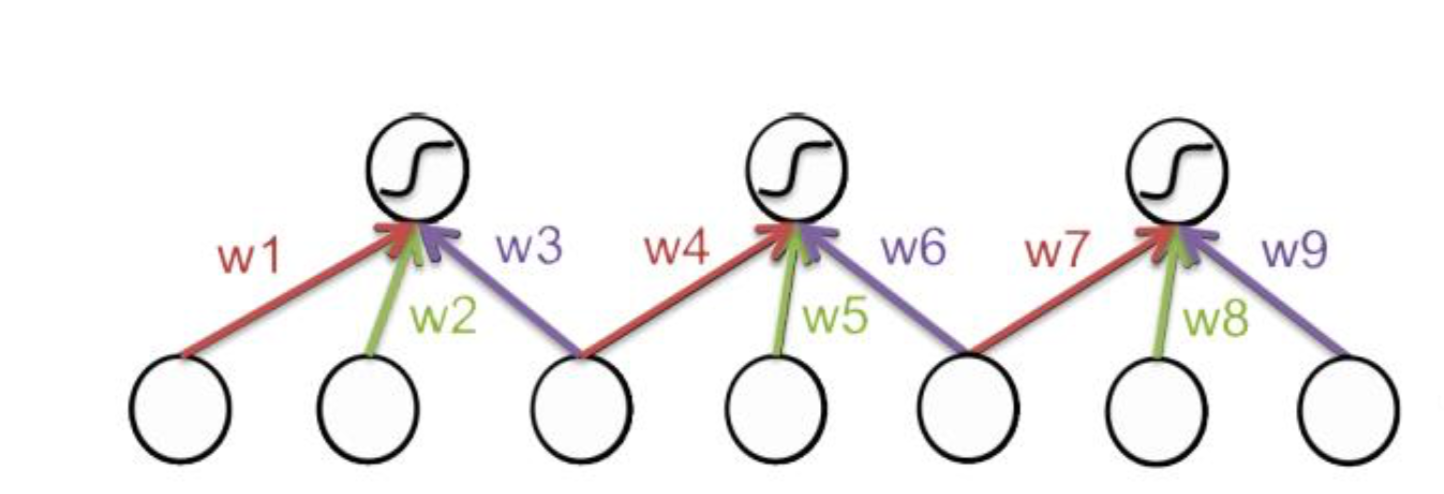
\includegraphics[scale=0.42]{cnn} 
\end{figure} 
Backpropagation in CNN, con $w_1 = w_4 = w_7$ \\
\[w_1 = w_{t-1} - \alpha (\frac{\partial \Lagr}{\partial W_1} + \frac{\partial \Lagr}{\partial W_4} + \frac{\partial \Lagr}{\partial W_7} ) \] \\
\[w_4 = w_{t-1} - \alpha (\frac{\partial \Lagr}{\partial W_1} + \frac{\partial \Lagr}{\partial W_4} + \frac{\partial \Lagr}{\partial W_7} ) \] \\
\[w_7 = w_{t-1} - \alpha (\frac{\partial \Lagr}{\partial W_1} + \frac{\partial \Lagr}{\partial W_4} + \frac{\partial \Lagr}{\partial W_7} ) \] \\

Calcolare numero di learning parameters nei livelli convolutivi\\
\[ input * output + bias \] \\
input = \# canali o filtri dell livello precedente \\
output = w del filtro * h del filtro \\
bias = \# dei filtri \\ \\
nella pratica
\[(w*h*previousFilters)+1)*correntFilters \] \\ \\
I layer pooling non hanno parametri \\ \\
Fully Connected layer parameters \\
\[ ((previousLayerParameters * 1 + 1) * neurons) \] \\ \\
Se si passa da un layer convolutivo o pool a uno fully connected si deve calcolare quanti parametri ha la matrice dell'immagine dopo le varie convoluzioni. \\


\clearpage

\subsubsection{ResNet}
\begin{figure}[h] 
\centering 
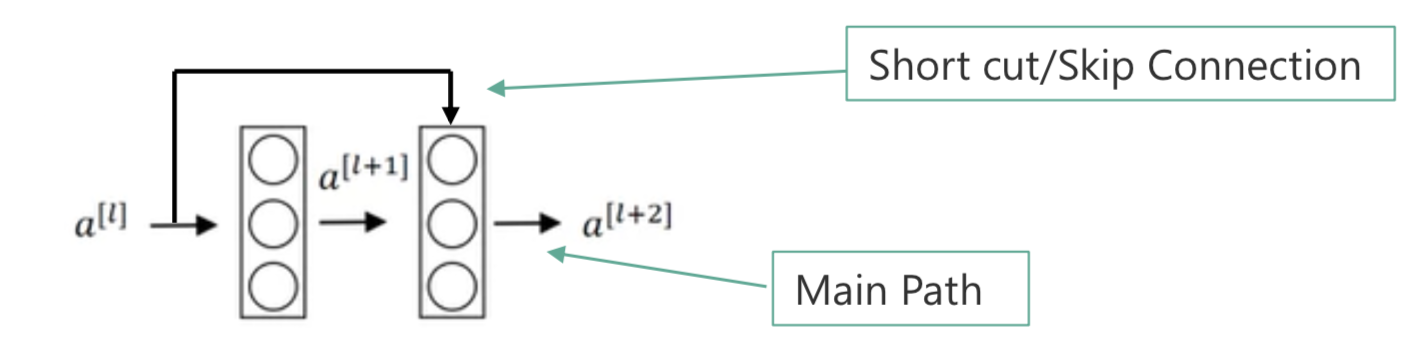
\includegraphics[scale=0.5]{resnet} 
\end{figure} 
\[ a^{l+2} = g((W_2 a^{l+1} + b_2) + a^l)\]

%----------------------------------------------------------------------------------------

\subsection{Attention Models}
Attention formula\\
\[ Attention(Q, K, V) = softmax(\frac{QK^T}{\sqrt{d_k}})V\]
con \\
$ x = $ matrice dopo il positional encoding \\
$ Q = x * W_Q $ \\
$ K = x * W_K $ \\
$ V = x * W_V $ \\ \\

Il prodotto $QK^T$ viene fatto con la seguente formula\\
\[ cos(v_i, u_j)||v_i|| ||u_j|| \]
con \\
$v_i$ elemento di Q \\
$u_j$ elemento di K

\subsection{Recurrent Neural Networks}
\subsubsection{Vanilla RNN}
\begin{figure}[h] 
\centering 
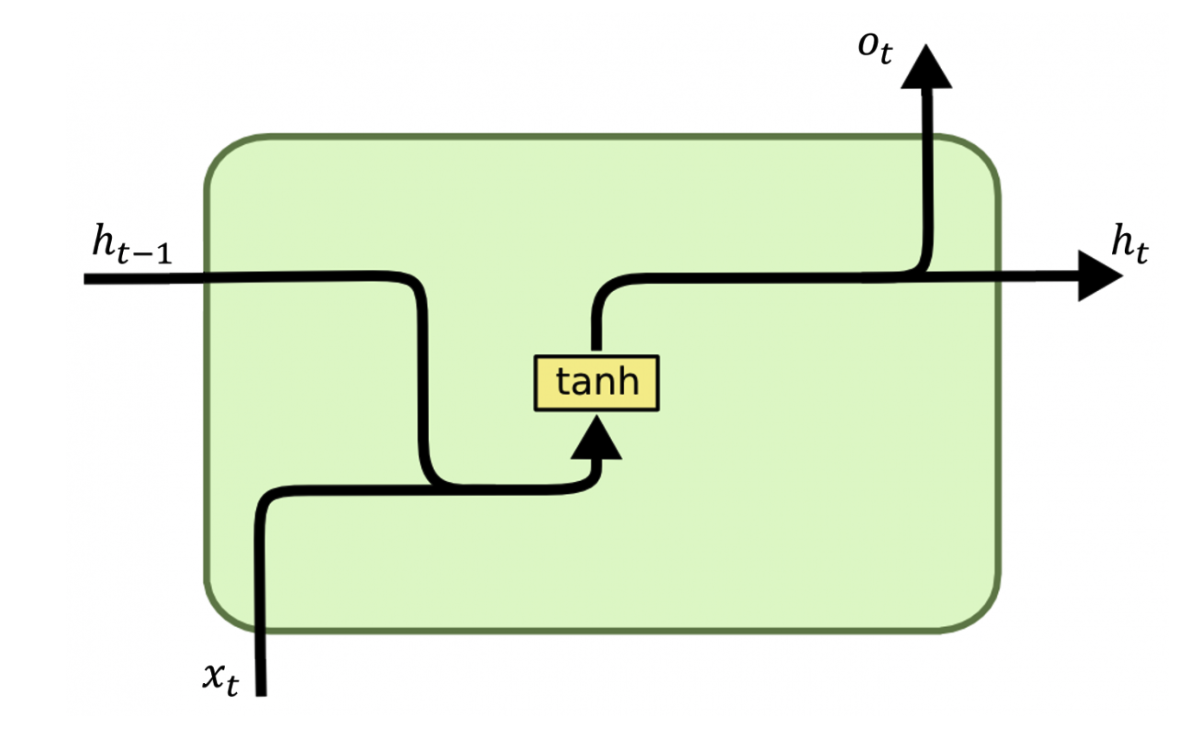
\includegraphics[scale=0.4]{vanilla} 
\end{figure} 
\[ a^{<t>} = tanh(W_a[a^{<t-1>}, x^{t}]+b_a) \]
con $a = h$ $\hat{y} = \sigma(W_ya^{<t>} +b_y)$\\

\subsubsection{Full GRU RNN}
\begin{figure}[h] 
\centering 
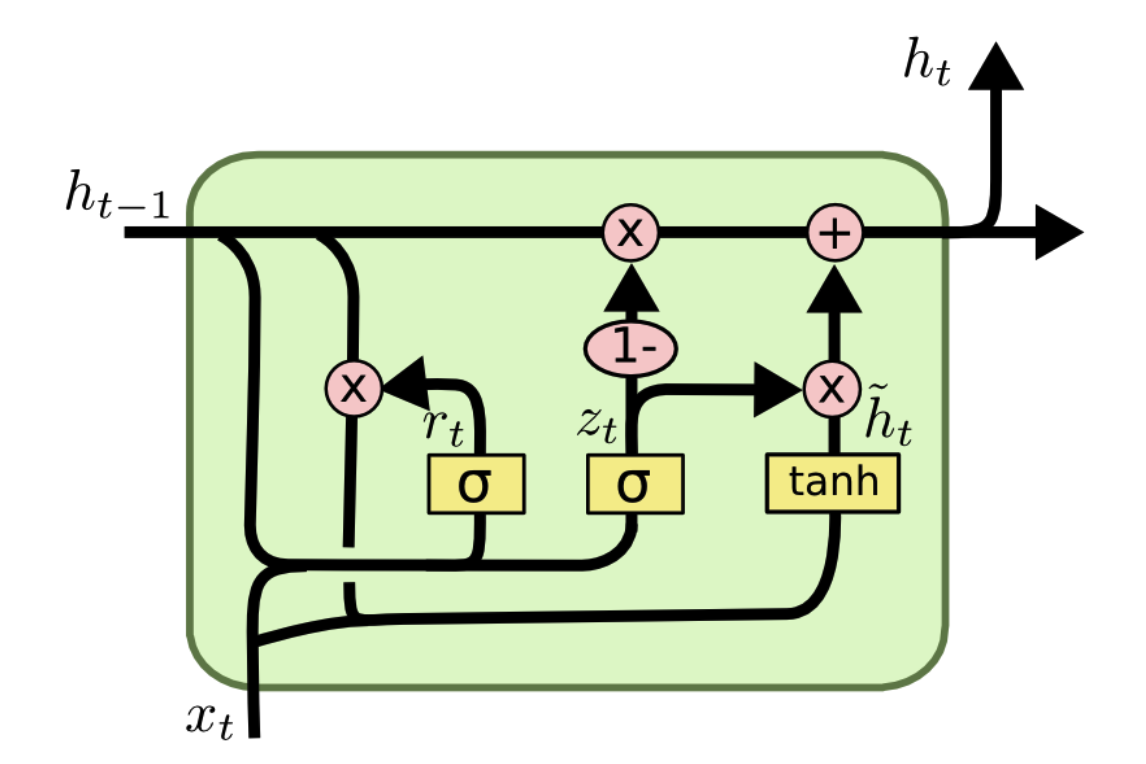
\includegraphics[scale=0.4]{gru} 
\end{figure} 
\[ \tilde{c}^{<t>} = tanh(W_c[\Gamma_r *{c}^{<t-1>}, {x}^{<t>}] +b_c) \]
\[ \Gamma_u   = \sigma(W_u[{c}^{<t-1>}, {x}^{<t>}] + b_u) \]
\[ \Gamma_r   = \sigma(W_r[{c}^{<t-1>}, {x}^{<t>}] + b_r) \]
\[ c^{<t>} = \Gamma_u * \tilde{c}^<t> + (1-\Gamma_u)*c^{<t-1>} \]
\[a^{<t>} = c^{<t>} \]
con $c = h$, $r_t = \Gamma_r$ e $z_t = \Gamma_u$ 


\subsubsection{LSTM}
\begin{figure}[h] 
\centering 
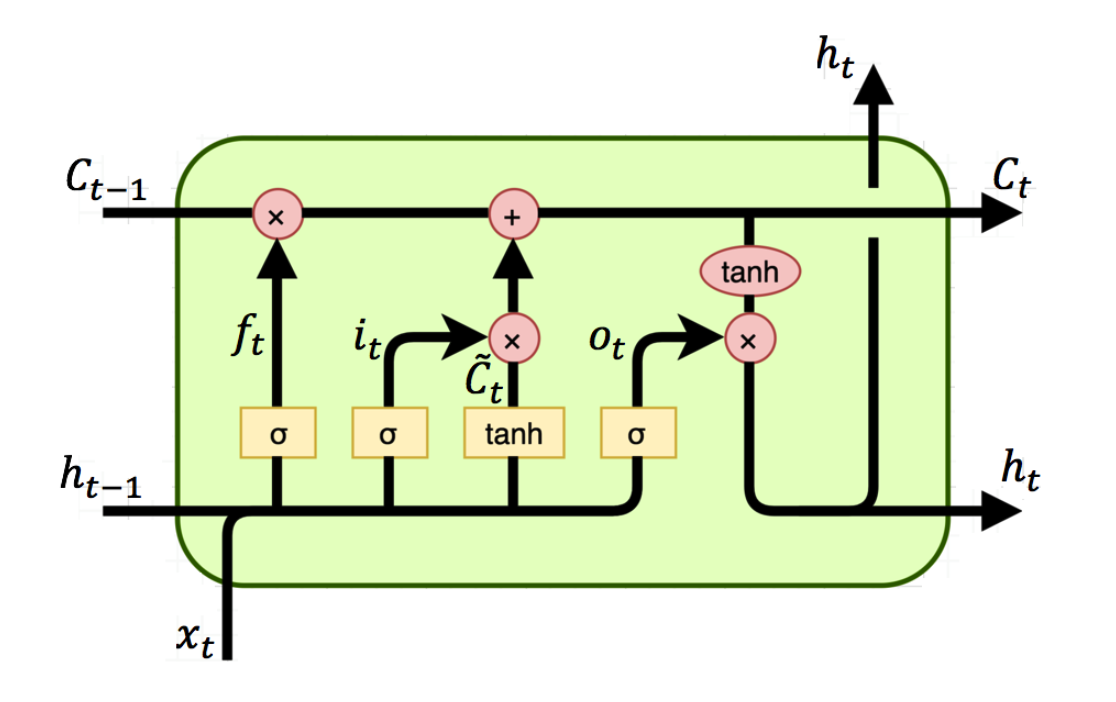
\includegraphics[scale=0.42]{lstm} 
\end{figure} 
\[ \tilde{c}^{<t>} = tanh(W_c[{a}^{<t-1>}, {x}^{<t>}] +b_c) \]
\[ \Gamma_u   = \sigma(W_u[{c}^{<t-1>}, {x}^{<t>}] + b_u) \]
\[ \Gamma_f   = \sigma(W_f[{c}^{<t-1>}, {x}^{<t>}] + b_f) \]
\[ \Gamma_o   = \sigma(W_o[{c}^{<t-1>}, {x}^{<t>}] + b_o) \]
\[ c^{<t>} = \Gamma_u * \tilde{c}^{<t>} + \Gamma_f*c^{<t-1>} \]
\[a^{<t>} = \Gamma_o * c^{<t>} \]

%----------------------------------------------------------------------------------------

\subsection{Generative Adversarial Networks}
Discriminator Loss\\
\[ minV(D) = E_{x\sim P_{data}(x)}[logD(x)] + E_{z\sim p_{z} (z)} [log(1-D(G(z)))] \]

Generator Loss\\
\[ E_{z\sim p_{z} (z)} [log(1-D(G(z)))] \]

con\\
$z$ è il rumore di input \\
$G(z)$ il risultato del generatore\\
$D(G(z))$ il risultato del discriminatore\\
$E_x$ il valore atteso considerando tutti i dati reali(grand truth del discriminatore)\\
$E_z$  il valore atteso considerando tutti i dati reali del generatore(grand truth del generatore)\\\\

Ricordo che è un minMAX game e che se la accuracy dal generatore raggiunge il 100\% il discriminatore arriva al massimo al 50\% (con fake sample perfetti deve tirare a caso)

%----------------------------------------------------------------------------------------


\subsection{Graph Convolutional Networks}
L'unica formula è\\
\[ \hat{A} = (\tilde{D}^{\frac{1}{2}}*\tilde{A})*\tilde{D}^{\frac{1}{2}} \] \\ \\
e di conseguenza\\
$ z = ReLU(W_0*X'_0*\hat{A} ) $ nell'hidden layer e $ z_n = Softmax(W_n*X'_{n}*\hat{A} ) $ nell'output layer\\

con \\ 
$\tilde{D} = $ la matrice dei gradi sommata ad $I$ alla $-1$ \\
$\tilde{A} = $ la matrice di adiacenza del grafo sommata a $\lambda I$\\



\end{document}
